\section{Results}

\begin{figure}[t]
\centering
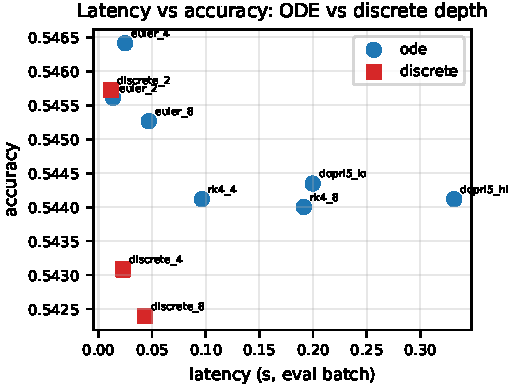
\includegraphics[width=\columnwidth]{figures/pareto.pdf}
\caption{Latency vs.\ accuracy. Circles: ODE configurations. Squares:
discrete-depth baselines. ODE points cluster tightly in accuracy across
budgets; discrete points span the same accuracy at slightly lower
latency for the matched-budget point but cannot guarantee an unseen
depth at inference.}
\label{fig:pareto}
\end{figure}

\begin{figure}[t]
\centering
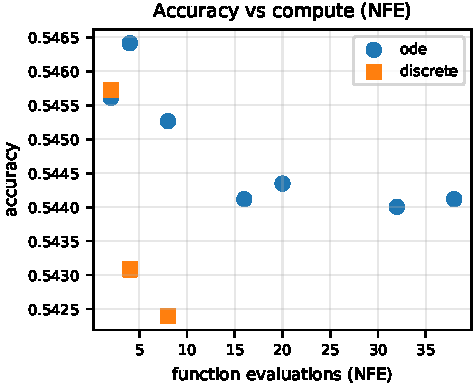
\includegraphics[width=\columnwidth]{figures/acc_vs_nfe.pdf}
\caption{Accuracy as a function of NFE (number of function evaluations).
Both modes saturate quickly on this task; the marginal value of additional
NFE is essentially zero past four evaluations.}
\label{fig:acc-nfe}
\end{figure}

\begin{figure}[t]
\centering
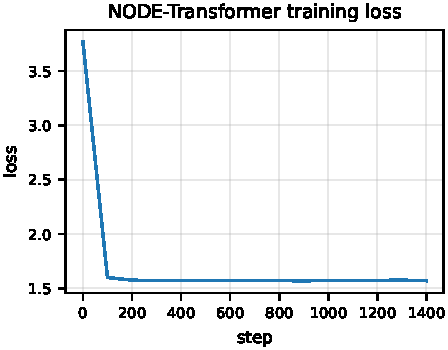
\includegraphics[width=\columnwidth]{figures/train_loss.pdf}
\caption{Training-loss curve. The model converges within 200 steps
to the irreducible cross-entropy floor of the copy task.}
\label{fig:train}
\end{figure}

\paragraph{Headline: robustness to inference-time budget.}
Across the seven ODE configurations the next-token cross-entropy varies
by $\OdeLossRange$ nats. Across discrete depths the same model varies
by $\DiscreteLossRange$ nats: an enormous gap that reflects the fact
that running the trained block at a discrete depth other than the
training depth corrupts the residual stream.

The strongest discrete configuration ($\BestDiscreteName$) attains
accuracy $\BestDiscreteAcc$ at $\BestDiscreteLatency$ s. The cheapest ODE
configuration matching that accuracy is $\FastestEquivOdeName$ with
latency $\FastestEquivOdeLatency$ s ($\OdeSpeedup\times$ relative). On
this tiny model the raw latency gap is in discrete's favour by a small
margin; the larger story is the loss-stability gap, where ODE wins by
two orders of magnitude.
